\bigskip

\textbf{Partie A}
 
 \begin{enumerate}
\item  	

	\hfill~
			
			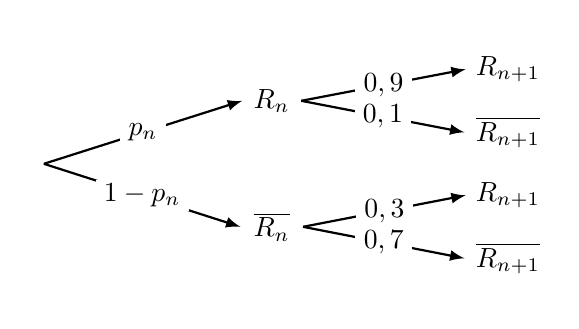
\begin{tikzpicture}[xscale=1,yscale=1,baseline=(R)]
				
				\tikzstyle{fleche}=[->,>=latex,thick]
				\tikzstyle{noeud}=[fill=white,circle,inner sep=2pt]
				\tikzstyle{feuille}=[fill=white,circle,inner sep=2pt]
				\tikzstyle{etiquette}=[midway,fill=white, inner xsep=3pt, inner ysep=1.5pt]
				
				\def\DistanceInterNiveaux{3}
				\def\DistanceInterFeuilles{0.8}
				
				\def\NiveauA{(0)*\DistanceInterNiveaux}
				\def\NiveauB{(1)*\DistanceInterNiveaux}
				\def\NiveauC{(2)*\DistanceInterNiveaux}
				\def\InterFeuilles{(-1)*\DistanceInterFeuilles}
				
				\node[noeud] (R) at ({\NiveauA},{(1.5)*\InterFeuilles}) {};
				\node[noeud] (Ra) at ({\NiveauB},{(0.5)*\InterFeuilles}) {$R_n$};
				\node[feuille] (Raa) at ({\NiveauC},{(0)*\InterFeuilles}) {$R_{n+1}$};
				\node[feuille] (Rab) at ({\NiveauC},{(1)*\InterFeuilles}) {$\overline{R_{n+1}}$};
				\node[noeud] (Rb) at ({\NiveauB},{(2.5)*\InterFeuilles}) {$\overline{R_n}$};
				\node[feuille] (Rba) at ({\NiveauC},{(2)*\InterFeuilles}) {$R_{n+1}$};
				\node[feuille] (Rbb) at ({\NiveauC},{(3)*\InterFeuilles}) {$\overline{R_{n+1}}$};
				
				\draw[fleche] (R.east)--(Ra.west) node[etiquette] {$p_n$};
				\draw[fleche] (Ra.east)--(Raa.west) node[etiquette] {$0,9$};
				\draw[fleche] (Ra.east)--(Rab.west) node[etiquette] {$0,1$};
				\draw[fleche] (R.east)--(Rb.west) node[etiquette] {$1 - p_n$};
				\draw[fleche] (Rb.east)--(Rba.west) node[etiquette] {$0,3$};
				\draw[fleche] (Rb.east)--(Rbb.west) node[etiquette] {$0,7$};
			\end{tikzpicture}
	\hfill~
		

\item Les évènements $R_n$ et $\overline{R_n}$ partitionnent l'univers, la loi des probabilités totales donne :

$p_{n+1} = P(R_{n+1}) = P\Big(R_n \cap R_{n+1}\Big) + P\Big(\overline{R_n} \cap R_{n+1} \Big) = p_n \times 0,9 + (1-p_n) \times 0,3 = 0,9p_n + 0,3 - 0,3p_n $

Donc on a bien $p_{n+1} = 0,6p_n + 0,3$ : on a donc bien établi la relation de récurrence annoncée.

\item
\begin{enumerate}
\item  Établissons la relation de récurrence de la suite $(u_n)$. Soit $n$ un entier naturel :

$\begin{aligned} u_{n+1} &= p_{n+1} - 0,75 \quad \text{par définition de la suite } (u_n)\\
				&= (0,6p_n + 0,3) - 0,75 \quad \text{par la relation de récurrence de la suite } (p_n)\\
				&= 0,6p_n - 0,45\\
				&= 0,6(u_n + 0,75)-0,45\quad \text{par définition de la suite } (u_n)\\
				&=0,6u_n+0,45-0,45\\
				&= 0,6u_n \\ \end{aligned}$

				La relation de récurrence de la suite $(u_n)$ est donc bien celle d'une suite géométrique, de raison $q = 0,6$. Le premier terme de la suite est $u_0 = p_0 - 0,75 = 0,6 - 0,75 = - 0,15$.
\item On peut donc donner la forme explicite du terme général de la suite géométrique :

$\forall n \in \N, \quad u_n = u_0 \times q^n = -0,15\times 0,6^n$.

On en déduit : $u_n = p_n - 0,75 \iff p_n = u_n + 0,75 = 0,75 - 0,15\times 0,6^n.$
\[\red p_n = 0,75 - 0,15\times 0,6^n.\]
\item La raison de la suite géométrique $u$ est comprise entre $-1$ et 1, strictement, donc la suite $u$ converge vers 0.

Par limite de la somme, on en déduit que la suite $p$ converge vers $\ell=0,75$.
\item En assimilant les probabilités à des proportions,  au bout d'un certain temps,  l'athlète franchira la barre  dans 75\,\% des cas.
\end{enumerate}

\end{enumerate}

\textbf{Partie B}

\begin{enumerate}
\item Ici, nous avons :
\begin{itemize}
\item une expérience à deux issues  dont le succès est \og l'athlète  franchit la haie \fg{} a une probabilité $p = 0,75$;
\item cette expérience est répétée dix fois (la course comporte 10 haies) d'une façon assimilable à une répétition identique et indépendante , donc $n=10$ répétitions;
\item dans ce schéma de Bernoulli de paramètres $n=10$ et $p=0,75$, on note $X$ la variable aléatoire qui compte le nombre de succès (le nombre de haies franchies pendant la course).
\end{itemize}
Avec ces éléments, on peut dire que $X$ suit la loi binomiale $ \mathcal{B}\left(10 ~;~ 0,75\right) $.
\item La probabilité demandée est $P(X = 10)$. Par propriété, on a :

$\displaystyle P(X=10) = \binom{10}{10} \times 0,75^{10} \times 0,25^0 = 0,75^{10}\approx 0,056$.

La probabilité que l'athlète franchisse les dix haies est donc d'environ  0,056.

\item  La probabilité demandée est $P(X \geqslant 9)$.

Selon le modèle de calculatrice, on peut obtenir une valeur approchée de ce résultat directement, ou alors on a recours à : $P(X \geqslant 9) = 1 - P(X <9) = 1 - P(X \leqslant 8)$.

La calculatrice donne une valeur approchée au millième près qui est 0,244.
\end{enumerate}

\bigskip
